\section{Conceitos Preliminares}
	%colocar definicao de workflows e diferença entre workflows de negocio e 		cientificos. OK
	%Tipos de fluxos de dados OK		
	\subsection{Workflows científicos}
		
		O termo workflow tem sua origem ligada a processos de automação de escritórios  que surgiram na década de 70. Com o objetivo de de gerar uma tecnologia capaz de fornecer uma base de apoio à distribuição de documentos nos escritórios, o que resultou na diminuição do uso de papéis\cite{Ogasawara2011}. Embora a sua origem esteja mais relacionada com a automação de tarefas de logística, essa teoria foi expandida para outras áreas do conhecimento, como Economia, Administração, até mesmo Física, Biologia e Oceanográfica. Segundo \textit{Workflow Management Coalition\cite{WfMC} , um workflow pode ser definido como: "A automação de um processo de negócio, completo ou apenas parte dele, através do qual documentos, informações ou tarefas são transmitidos de um participante a outro por ações, de acordo com regras procedimentais"}.

		Já o termo workflow científico está bem mais ligado com as ciências do que o termo workflow, por ter o seu foco na manipulação de dados e na execução de tarefas que estão diretamente relacionadas com o processamento de dados. Essa grande utilização de dados caracteriza os workflows científicos como uma estrutura baseada no fluxo de dados, ou seja, as conexões entre as atividades representam o fluxo de dados.\cite{Teixeira2013}
		 
		Os sistemas de workflows científicos geralmente são compostos por um grande número de tarefas que podem depender dos dados produzidos por outras tarefas. Essas tarefas podem ser manuais ou automáticas e são responsáveis pela gerência de todo o ciclo de vida do experimento científico: composição, mapeamento, execução e análise. Cada etapa do ciclo do experimento é muito importante e precisa ser analisada com cuidado\cite{Junior2012}:

	\begin{itemize}
		\item Composição: especificações das tarefas que compõem o experimento, dos tipos de dados de entrada e saída e das dependências de dados existentes entre as atividades e o ambiente computacional em que o workflows será executado.
		
		\item Mapeamento: associação do modelo de workflow com os recursos computacionais disponíveis.		
		
		\item Execução: realização das tarefas definidas anteriormente no ambiente computacional.

		\item Análise: estudo dos dados gerados na execução.

	\end{itemize}


		Todo esse processo pode ser automatizado de forma que o cientista possa reexecutá-lo até que os dados obtidos na fase de análise sejam os dados esperados. 
		
		A estrutura de um workflow é composta pelas atividades a serem executadas e as conexões entre elas. Compreende-se por atividade cada ação realizada que recebe um dado de entrada e produz um dado ou uma informação de saída. O conjunto de conexões entre as atividades pode ser caracterizado como fluxo de controle ou fluxo de dados. Neste trabalho estamos interessados em analisar apenas o fluxo de dados, pois é a estrutura que está mais interligada com os workflows científicos . O fluxo de dados representa a dependência entre as atividades e os dados manipulados, e a forma como os dados são utilizados no workflow, com atividades produzindo dados que serão consumidos por outras atividades\cite{Teixeira2013}. 

		As principais construções de fluxo de dados são\cite{Teixeira2013}:
		
	\begin{itemize}
		\item \textit{Pipeline}: são várias atividades combinadas sequencialmente, em que cada atividade recebe como entrada os dados produzidos como saída da atividade anterior;  

		\item \textit{Distribuição de dados(Date Partitioning)}: é feita por atividades que produzem dados de saída que são recebidos como entrada por múltiplas atividades, ou que apenas particionam grandes conjuntos de dados em subconjuntos menores para serem processadas por outras atividades;
		
		\item \textit{Agregarão de dados(Date Agregation)}: é feita por atividades que processam múltiplos conjuntos de dados de entrada, gerando uma combinação dos dados como saída;
		
		\item \textit{Redistribuição de dados}: é feita por atividades que funciona como um ponto de sincronização com relação ao processamento de dados, recebendo como entrada várias porções de dados e produzindo também múltiplas saídas como resultado.
	\end{itemize}
		
	Veja a figura~\ref{fig:RGRP} alguns exemplos gráficos de fluxo de dados.
			
		%caractericao geral dos gerenciadores kepler, taverna.
		%falar depois do Pegasus e do DAX que utilizado pelo pegasus, o motagem é feito em cima do formato DAX.
	\subsection{Sistemas gerenciadores de workflows científicos}
		Para apoiar os workflows científicos, diversos Sistemas de Gerencia de Worflows Científicos(SGWfC) foram desenvolvidos. Onde cada um deles apresentam uma particularidade para representação dos workflows e visa atender determinados tipos de aplicações de áreas específicas. Estes SGWfC são responsáveis pela coordenação das chamadas a programas, seja em ambiente local ou para ambientes distribuídos\cite{Ogasawara2011}. Os Sistemas mais utilizados , segundo o numero de workflows compartilhados no \textit{myexperiement}\footnote{url="http://www.myexperiment.org/", repositório de workflows científicos},estão descritos, de maneira bem básica, logo abaixo:
		\subsubsection{Taverna}
				O Taverna foi desenvolvido como parte do projeto \textit{mygrid}\footnote{http://www.mygrid.org.uk/}, é um ambiente para modelagem, execução e análise de workflows científicos, tem como foco principal aparar cientistas da área de Ciências Biológicas que normalmente não possuem conhecimento profundo de computação. O Taverna tem código aberto o que permite unir projeto de terceiros\cite{Teixeira2013}.

				Um workflow no Taverna é especificado como um grafo direcionado onde os nós, chamados de processadores,  são as atividades e representam componentes de software. Um nó processador consome dados que chegam nas suas entradas e produzem dados de saída. Cada arco no grafo conecta um entrada com uma saída de dados e expressa uma dependência entre as atividades o que denota o fluxo de dados entre as atividades\cite{Teixeira2013}.
				
	A construção e execução dos workflows no Taverna é feita com o auxilio de uma interface gráfica, que é  representado posteriormente na linguagem Scufl(\textit{Simplified Conceptual Workflow Language}) que descreve o workflow em um formato baseada em XML e depois é executado pelo \textit{Motor de Execucão}\cite{Teixeira2013}. Observe a seguir uma imagem dessa interface gráfica:
				
		\begin{figure}[!h]
			\centering
			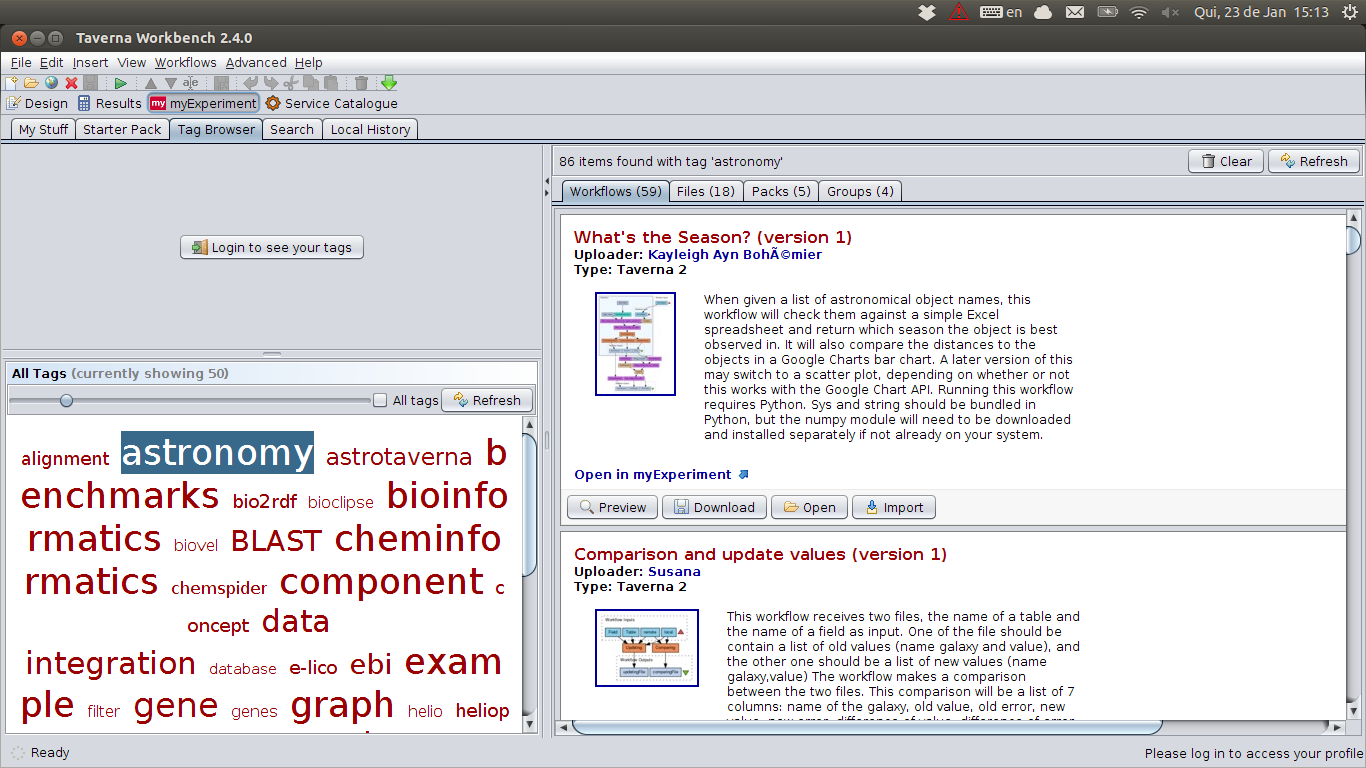
\includegraphics[width=1.1\textwidth]{img/taverna.png}
			\caption{Interface gráfica do Taverna}
		\end{figure}
		
		A linguagem Schfl possui uma serie de componentes que permite a representar no seu formato todo o workflow. A construção mais básica do Taverna são os \textit{Pipelines}, porém é possível criar construções de fluxos de dados como Agregação, Distribuição e Redistribuição de dados \cite{Teixeira2013}.
 	
 		Como pode ser visto na figura acima o Taverna possui uma integração com o \textit{myexperiment} para compartilhamento dos workflows modelados nele. O que talvez tenha o tornado um dos SGWC mais conhecidos, além de todo seu poder de construção de workflows científicos voltado para área Biológicas.
		
		\subsubsection{Pegasus}
		
		O SGWC Pegasus é um \textit{framework} que permite o mapeamento de instâncias de workflows em um conjuntos de recursos distribuídos, como uma grade. A descrição de um workflow no Pegasus é feita a partir de uma arquivo de entrada na forma de um DAG em formato XML, na linguagem DAX(\textit{Directed Acyclic Graph in XML}), que representa todo o fluxo de processamento e as dependências entre as tarefas, além dos recursos computacionais em que o workflow será executado\cite{Teixeira2013}.
		
		O DAX descreve os workflows termos de atividades, onde cada atividade consiste de um código de identificação da atividade, os nomes dos arquivos de entrada e saída de dados e uma relação de dependência entre as atividades. A partir dessa definição de dependências é possível construir as principais estruturas de fluxos de dados, \textit{pipelines}, distribuição, agregação e redistribuição de dados. O DAX também permite a definição de vários arquivos de saída que podem ser de tipos diferentes, dependo da necessidade da atividade\cite{Teixeira2013}. 
		
		 Código abaixo mostra como é representada uma atividade na linguagem DAX\footnote{https://confluence.pegasus.isi.edu/display/pegasus/WorkflowGenerator, Este exemplo foi retirado do DAX que representa o Montage}:
		

\begin{lstlisting}[language=XML, caption=Exemplo de uma atividade DAX]

<job id="ID000002" namespace="vahi" name="findrange" version="1.0" 
level="2"dv-namespace="vahi" dv-name="left"	dv-version="1.0">
	<argument>
		-a left -T 6 -i 
		<filename file="f.b1"/> -o <filename file="f.c1"/>
		-p 0.5
	</argument>
	<uses file="f.b1" link="input" dontRegister="false" dontTransfer="false" temporaryHint="true"/>
	<uses file="f.c1" link="output" dontRegister="true" dontTransfer="false" temporaryHint="true"/>
</job>

\end{lstlisting}

	Numa próxima fase o DAX é mapeado pelo Pegasus e as atividades definidas são executadas.
	
%colocar a definicao formal de redes de Petri, pegar na dissertacao da professra Kelly		OK
% se der tempo falar mais sobre redes de petri temporizadas e estocásticas
	\subsection{Redes de Petri}
		As Redes Petri(RdP) é um dos formalismos mais utilizados para modelagem analítica e análise de sistemas concorrentes mais utilizados,isso deve-se à fácil compreensão representação gráfica e devido ao seu potencial matemático para análise de modelos. Algumas características importantes de workflows científicos pôde ser facilmente representadas utilizando RdP, tais como a sincronização de tarefas, concorrência e controle de dependências\cite{Braghetto2011}.
		Uma RdP pode ser formalmente definida pela tupla $RdP={L,T,A,P,m_{0}}$, em que:
		\begin{itemize}
		\item $L=\{l_{1},l_{2},...,l_{L}\}$ é um conjunto de lugares;
		\item $T=\{t_{1},t_{2},...,t_{T}\}$ é um conjunto de transições;
		\item $A\subseteq(L x T)\bigcup (TxL)$ é um conjunto de arcos;
		\item $P: A \rightarrow \mathbbm{N}$ é a função peso dos arcos;
		\item $m_{0}=\{m_{01},m_{02},...,m_{0L}\}$ é a marcação inicial da rede;
		\end{itemize}
		
		Cada um dessas definições está associados a diferentes e importantes conceitos de RdP, que são:
		
			\begin{itemize}

				\item \textit{lugar} (representado graficamente por um círculo)- modela uma condição que deve ser satisfeita para que o disparo da transição seja realizado;

				\item \textit{transição} (representado graficamente por um retângulo) - pode ser compreendido por uma por uma acao ou um evento;

				\item \textit{arco orientado} liga um lugar a uma transição ou o contrário, ligando condições e eventos;

				\item \textit{fichas, marcas ou tokens} (representado por um ponto preto)- Representam um recurso ou um estado de um sistema;

				\item \textit{peso} - os arcos possuem um peso associado a eles; os pesos indica quantas fichas uma transição consome de um lugar de entrada ou quantas fichas uma transição acrescenta em um lugar de saída. Por \textit{default} quando um arco não possui um peso o peso é 1;
					
			\end{itemize}
			
			Da necessidade de modelagem de sistemas grandes e complexos, como os encontrados na natureza e na sociedade, foram definidas sobre a base de Redes de Petri clássica outras redes de alto nível, como as Redes de Petri Temporizadas(RdPTs) e Redes de Petri Estocásticas(RdPEs). As RdPTs como o nome diz permite modelar situações que ocorrem entre o início e fim de cada tarefa em termos do tempos. O permitiu diferentes possibilidades para modelagem, como lugares temporizados, fichas temporizadas e todas as outras estruturas descritas acima puderam ser tempodizadas e permitiram modelar uma série de sistemas reais. Já as RdPEs é uma subclasse das RdPTs, onde o tempo de atraso de uma transição é uma variável aleatória exponencialmente distribuída\cite{Braghetto2011}. 
		
	Ao se usar as redes de Petri para se modelar a execução de um workflow, cada vértice pode armazenar um ou mais tokens, os vértices de transição de redes de Petri podem consumir e produzir tokens de múltiplas localizações. Os vértices de transições agem em tokens de entrada por um processo denominado disparo. Quando uma transição é disparada, ela consome os tokens de suas posições de entrada, realiza alguma tarefa de processamento, e realoca um número específico de tokens nas suas posições de saída. Isso é feito atomicamente. Como os disparos são não-determinísticos, as redes de Petri são muito utilizadas para modelar comportamento concorrente em sistemas distribuídos. 	
			
		\subsubsection{PIPE}
			
			O PIPE\cite{PIPE} é uma ferramenta \textit{open source} criada para análise de RdPEs, possui uma interface gráfica simples e intuitiva. Com um conjunto de módulos para avaliar o comportamento estatístico das RdPEs, a representação de Lugares, Transições, Arcos e Fichas, segue o modelo gráfico descrito na seção anterior, como pode ser visto na figura abaixo:			
						
			\begin{figure}[h]
				\center
				\caption{Interface gráfica-PIPE}
				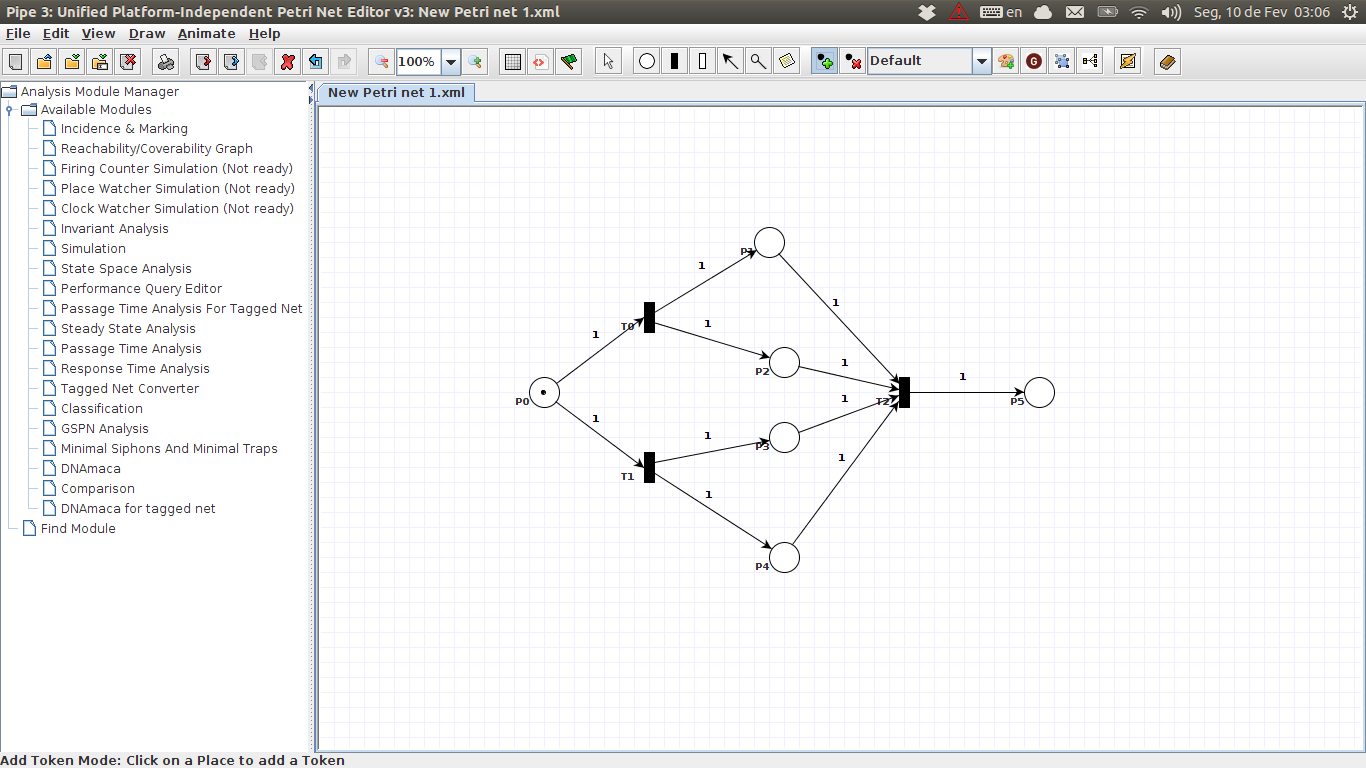
\includegraphics[width=1\textwidth]{img/pipe.jpg}
				\label{fig:PIPE}
			\end{figure}						
			
		Após a construção gráfica do modelo é possível observar a evolução dinâmica do sistema modelado e fazer a análise dos dados gerados, assim como exportar em formato XML ou o PNG da Rede Petri representada.